\begin{landscape}
	\begin{figure}[tb]
		\centering
%		\begin{adjustwidth}{-0.2\linewidth}{-0.2\linewidth}
%			\hspace{40pt}
			\begin{subfigure}[c]{.45\linewidth}
				\centering
				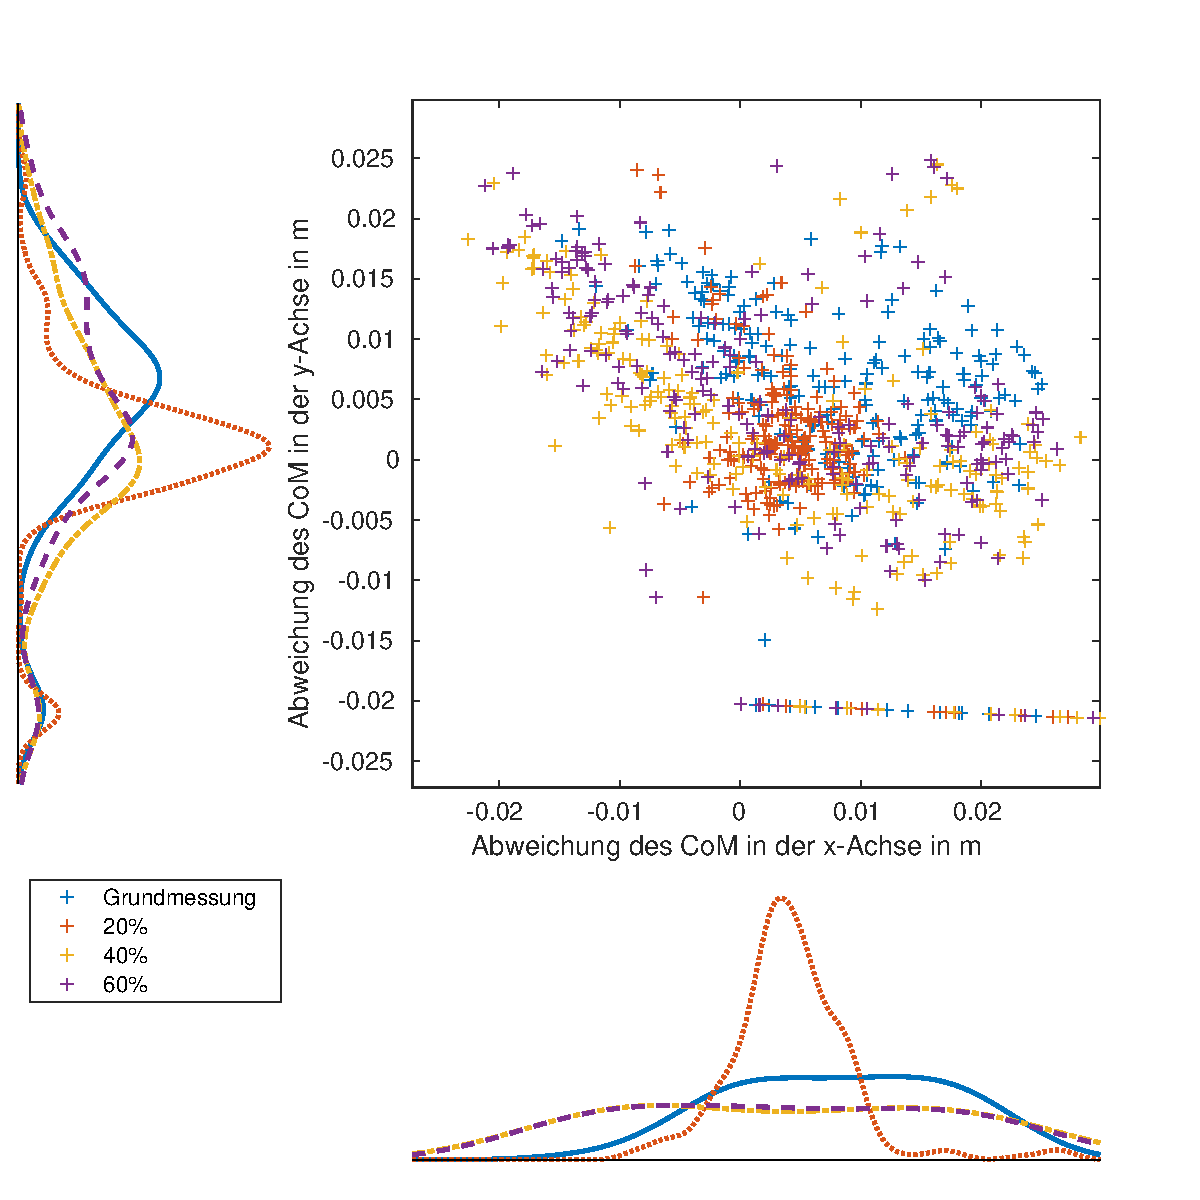
\includegraphics[width=\linewidth]{Bilder/links_CoM_ohneM.pdf}
				\caption{ohne Magneten}
%				\vspace{5pt}
			\end{subfigure}
%			\hspace{-10pt}
			\hfill
			\begin{subfigure}[c]{.45\linewidth}
				\centering
				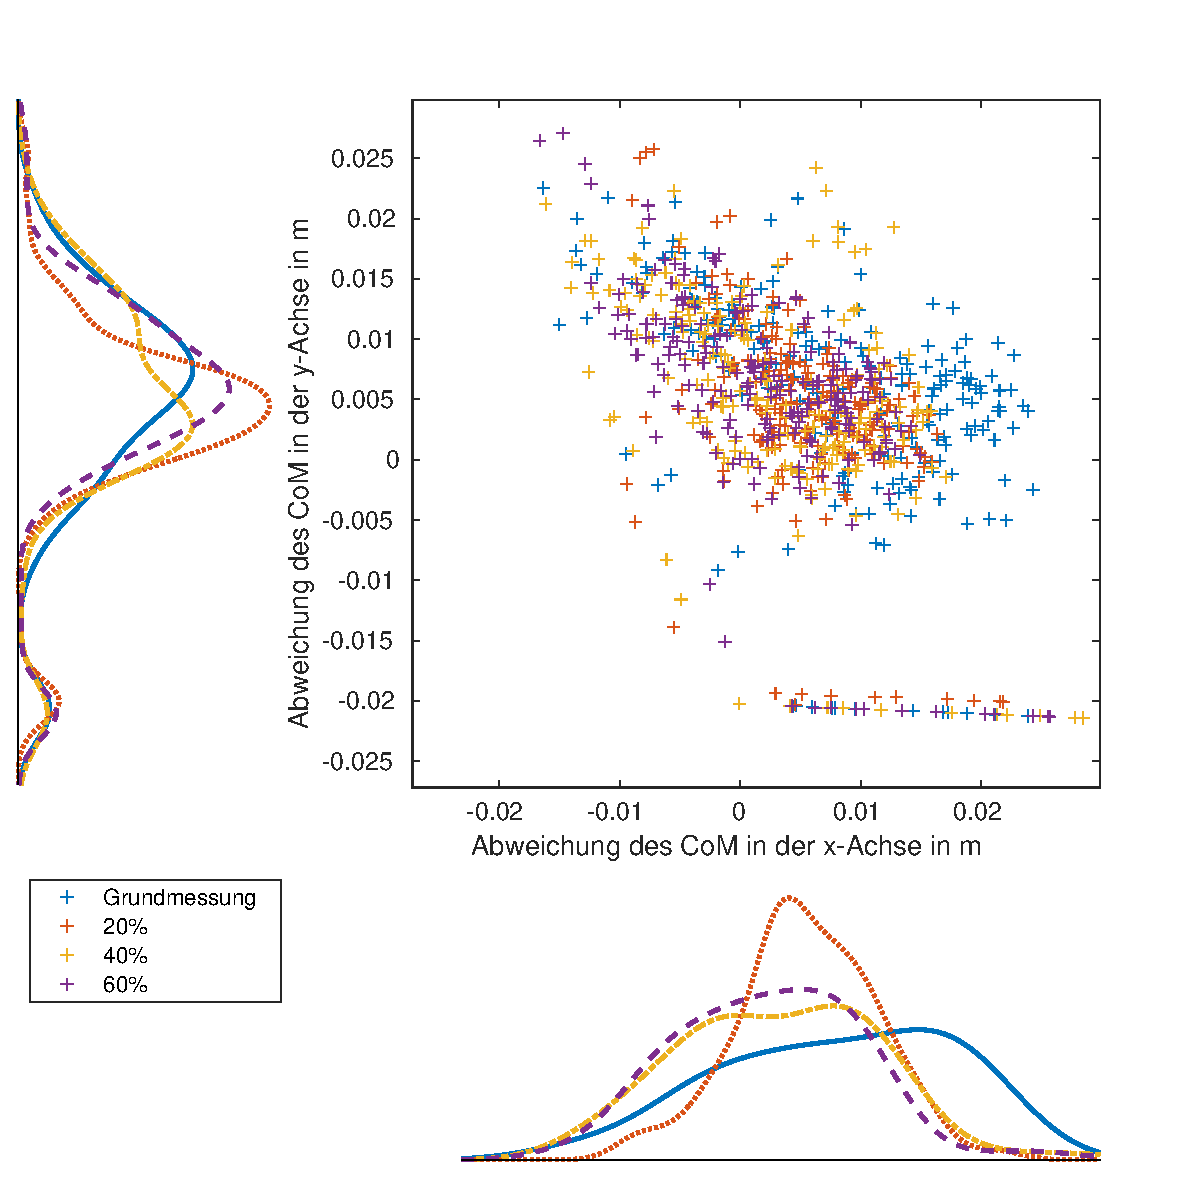
\includegraphics[width=\linewidth]{Bilder/links_CoM_mitM.pdf}
				\caption{mit Magneten}
%				\vspace{5pt}
			\end{subfigure}
%		\end{adjustwidth}
		\caption{Linker errechneter Massenschwerpunkt aufgenommen durch die FSR, x-Achse auf y-Achse mit jeweiliger Wahrscheinlichkeitsdichtefunktion} \label{CoM_links}
	\end{figure}
\end{landscape}